%%%%%%%%%%%%%%%%%%%%%%%%%%%
%%% Chapter definitions %%%
%%%%%%%%%%%%%%%%%%%%%%%%%%%
% Chapter title
\renewcommand{\mychaptertitle}{%
Controlling the secondary flows in\\ turbulent Taylor--Couette flow
% Span-wise varying roughness in highly turbulent\\ Taylor-Coutte flow
}
% Chapter short title
\renewcommand{\mychaptershorttitle}{%
Controlling the secondary flows in turbulent Taylor--Couette flow
% Span-wise varying roughness in turbulent Taylor-Coutte flow
}
% Chapter authors
\renewcommand{\mychapterauthors}{%
\textbf{Dennis~Bakhuis},
Rodrigo~Ezeta,
Pieter~Berghout,
Pim~A.~Bullee,
Dominic~Tai,
Daniel~Chung,
Sander~G.~Huisman,
Roberto~Verzicco,
Detlef~Lohse,
and
Chao~Sun
\textit{Controlling the secondary flows in turbulent Taylor--Couette flow using
spanwise varying roughness},
in preparation. Experiments are done by Bakhuis, Ezeta and Bullee. Numerical
simulations are done by Berghout. Analysis of PIV and LDA is done by Ezeta.
Analysis of the torque and LDA is done by Bakhuis. Writing is done by Bakhuis,
Ezeta, Berghout, Bullee, and Huisman. Supervision by Huisman, Chung, Verzicco,
Lohse and Sun. Proofread by everyone.
}
% Chapter abstract
\renewcommand{\mychapterabstract}{%
Highly turbulent Taylor--Couette flow with spanwise-varying roughness is
investigated experimentally and numeriacally to determine the effects of the
normalized axial size $\tilde{s}$ of roughness patches on the total drag on
the inner cylinder and the local flow structures. We apply sandgrain
roughness, in the form of alternating bands to the inner cylinder.
Numerically, the Taylor number is $\mathcal{O}(10^9)$ and $\tilde s$ is varied
such that $0.47\leq \tilde s \leq 1.24$ and is simulated using a direct
numerical simulation in conjunction with an immersed boundary method.
Experimentally, we explore $\text{Ta}=\mathcal{O}(10^{12})$ and $0.61\leq
\tilde s \leq 3.74$ in the Twente Turbulent Taylor--Couette facility
(T${}^3$C). For both approaches the radius ratio is fixed at $\eta = 0.716$.
We present how the flow scales with $\text{Ta}$ and how it depends on the
boundary conditions set by $\tilde s$. Both numerically and experimentally, we
find a maximum in the angular momentum transport when $\tilde s$ is varied. We
attribute this to the re-arrangement of the large-scale structures triggered
by the presence of the rough patches, which yields effectively, tuned
turbulent vortices with different axial wavelengths. We describe how the local
flow rearranges for varying $\tilde s$ and how these local effects are
reflected in the global response of the system.
}
\renewcommand{\mychaptermark}{Span-wise varying roughness}
\renewcommand{\mychapterlabel}{chap:spanwise}
\renewcommand{\mychaptericon}{fig/swchapter4.png}
%%%%%%%%%%%%%%%%%%%%%%%%%%%%%
%%% Create Chapter Header %%%
%%%%%%%%%%%%%%%%%%%%%%%%%%%%%
%%%%%%%%%%%%%%%%%%%%%%
%%% Chapter header %%%
%%%%%%%%%%%%%%%%%%%%%%
\globalcolor{ChapterText}
\chapter[\mychaptershorttitle]{%
    \mychaptertitle%
    \ifdefined\starwarsfootnotes
        \textsuperscript{%
            \hspace{-1mm}%
            \includegraphics[height=\swsymsize]{\mychaptericon}%
        }%
        \blfootnote{%
            \textcolor{footnotetextcolor}{%
                \textsf{%
                    \vspace{0.5mm}\hspace{-1mm}%
                    \includegraphics[height=\swfnsymsize]{\mychaptericon}%
                    \hspace{0.5mm}%
                    Based on: \mychapterauthors%
                }
            }
        }
    \else
        \footnote{\textsf{%
             Based on: \mychapterauthors%
        }}%
    \fi
}
\pagecolor{ChapterBackground}
\afterpage{\pagecolor{White}\globalcolor{Black}} 
\label{\mychapterlabel}
\chaptermark{\mychaptermark}
\noindent\rule{\textwidth}{0.4pt}%
\vspace{0.2cm}
\noindent\textsf{\mychapterabstract}
\clearpage

%%%%%%%%%%%%%%%%%%%%%%%%
%%%% end title page %%%%
%%%%%%%%%%%%%%%%%%%%%%%%
\graphicspath{{ChapterFive/fig/}}
%%%%%%%%%%%%%%%%%%%%%%%%%%%%%%%
%%%% Start of chapter data %%%%
%%%%%%%%%%%%%%%%%%%%%%%%%%%%%%%
\section{Introduction}\label{sec:spanwiseintro}
Many turbulent flows are bounded by irregular, rough, boundaries. These flows
are extensively studied, under the approximation that the roughness is
homogeneous \citep{Jimenez2004}. Homogeneously rough surfaces have a
characteristic length scale $k$ that is much smaller than the largest wall
normal length scale $\delta$. The effects of the roughness in these flows is
believed to be confined to the immediate vicinity of the wall (i.e. the
roughness sublayer), whereas in the outer, inertial, layer, the flow only
experiences the effective shear stress of the surface, i.e. Townsend's outer
layer similarity \citep{Townsend1976}. As such, the focus of many studies was
to find functional relationships between the parameters that describe both the
roughness geometry and the skin friction coefficient $C_f$ \citep{Flack2010}.
In practice, however, flows are bounded by rough boundaries that not only vary
on the scale of $k$, but also on a much larger scale $s$, where $s=O(\delta)$.
Whereas these variations can be either laterally (spanwise) or longitudinally
(streamwise), we focus here on the former.
Examples of these flows are found in shipping (i.e.~the formation of patches of biofouling on ship hulls \citep{Schultz2007}) and geophysical flows (e.g.~the atmospheric flows over spanwise-varying terrain \citep{Ren2011}).\\
\indent Hitherto, the research is focused on the effects of spanwise-varying rough surfaces on canonical systems of wall-bounded turbulence research, i.e. pipe flow \citep{Koeltzsch2002}, boundary layer flow \citep{Anderson2015} and channel flow \citep{Chung2018}.
The hallmark of flows over these surfaces is the presence of spanwise wall-normal secondary flows of the size  $O(\delta)$, with mean streamwise vorticity. Examples of studies where this has been observed are the works of \citet{Koeltzsch2002} on the effects of convergent and divergent grooves (reminiscent of shark skin) and the work by \cite{Wang2006} on spanwise-varying riverbeds. We note that earlier research dates back to the works of \citet{Hinze1967,Hinze1973} on the field of surface stress variations in duct flows.\\
\indent Following up on the work of \cite{Koeltzsch2002}, \cite{Nugroho2013} set out to perform a parametric study of the converging-diverging riblets surface in a zero pressure gradient BL. They find a thickening of the BL height above the converging regions, and a thinning of the BL height above the diverging regions. Furthermore, the energy spectra shows an increased energy content of the larger scales. \cite{Barros2014} performed stereo particle image velocimetry (PIV) in the spanwise wall-normal plane of the flow over a turbine blade replica and found spanwise variations of the order of $\delta$ in the mean velocity field. With the same configuration, \citet{Mejia-Alvarez2013} identified regions of low momentum pathways (LMPs) and high momentum pathways (HMPs) in the instantaneous fields. Here, LMPs coincide with regions of enhanced turbulent kinetic energy (TKE) and Reynolds shear stress (RSS), and rather remarkably, these regions do seem to occur at recessed roughness heights.
\cite{Willingham2014} found very similar behavior of the secondary flows for a much more regular surface geometry.
\cite{vanderWel2015} found that only when $s/\delta \gtrapprox 0.5$, where $s$ is the spacing between the streamwise aligned Lego\textsuperscript{\textregistered} blocks, secondary flow formation is observed. However, for $s/\delta \lessapprox 0.5$ the secondary flows are confined to the roughness sublayer. Interestingly, contrary to the findings of \citet{Mejia-Alvarez2013}, they find LMPs on top of their elevated blocks, and HMPs in between the roughness strips.
\cite{Yang2017}, however, found $s/H \gtrapprox 0.2$, with $H$ the channel half height, as the threshold for heterogeneous behavior of the streamwise aligned pyramid elements. By carefully assessing the terms in the transport equation of TKE, \cite{Anderson2015} found that spanwise variations of roughness leads to a local imbalance of production and dissipation of TKE, as already proposed by \cite{Hinze1967}.
Since the secondary flows are driven by a spatial gradient in the RSS, they find that the mean secondary flows are Prandtl's secondary flow of the second kind \citep{Bradshaw1987}.
\cite{Medjnoun2018} observed a breakdown of outer layer similarity in the local profiles of the mean flow, turbulent intensity, and the energy spectra, evidently induced by the presence of the secondary vortices.
Finally, \cite{Chung2018} studied the influence of the spacing of idealized (i.e. no geometric induced disturbances to the flow) regions of low shear stress and high shear stress.
They find that for $s/\delta \lessapprox 0.39$ the notion of outer layer similarity is retained.
Interestingly, for $s/\delta \gtrapprox 6.28$, they find a sign reversal of the isovels (stream velocity contour lines), with respect to the orientation of the secondary flows, that remain upwelling over low shear stress regions.\\ 
\indent The aforementioned studies were all carried out in systems that lack two characteristics which are intrinsic to many applications, namely the curvature in the streamwise direction (as in turbine blades), and the presence of strong secondary motions (as in the atmospheric boundary layer). A canonical system in which these two properties can be simultaneously observed is the Taylor--Couette (TC) flow.
TC flow is the flow in between two coaxially, independently rotating cylinders. Its geometry is characterized by the inner cylinder radius $r_{i}$, outer cylinder radius $r_o$, and the height of the cylinders $L$, captured by two dimensionless parameters; the radius ratio $\eta=r_i/r_o$ and the aspect ratio $\Gamma=L/d$, where $d=r_o-r_i$ is the gap in between the cylinders. 
Since TC is a closed system, one can directly relate global and local quantities through exact mathematical relations \citep{Eckhardt2007}. The driving in TC flow is expressed in dimensionless form by the Taylor number: 
%
\begin{align}\label{eq:Ta}
    \text{Ta} = \frac 14 \sigma d^2 \frac{(r_i+r_o)^2(\omega_i-\omega_o)^2}{\nu^2},
\end{align}
%
where $\omega_{i,o}$ are the inner and outer angular velocity of the cylinders respectively, $\nu$ is the kinematic viscosity, and $\sigma=\left(\left(1+\eta\right)/\left(2\sqrt{\eta}\right)\right)^4$ is the so-called geometric Prandtl number, in analogy to the Prandtl number in Rayleigh-B\'{enard} convection \citep{Eckhardt2007}. Alternatively, when the outer cylinder is at rest ($\omega_o=0$), the driving can also be expressed with a Reynolds number based on the outer scales $\text{Re}_i=r_i \omega_i d / \nu$. This Reynolds number and Ta (for $\omega_o=0$), are related by $\text{Re}_i = (8 \eta^2/(1 + \eta)^3) \sqrt{\Ta}$.
In TC flow, the angular velocity flux $J^\omega$ is radially conserved. Here, $J^\omega = r^3 (\langle u_r \omega \rangle_{A,t} - \nu  \frac{\partial}{\partial r} \langle \omega \rangle _{A,t})$, where the brackets $\langle \cdot \rangle _{A,t}$ denote averaging over a cylindrical surface and time. The angular momentum flux for the case of laminar flow is $J_{lam}^\omega = 2\nu r_i^2 r_o^2 (\omega_i-\omega_o) /(r_o^2 - r_i^2)$. In this way the response of the flow is  quantified with the dimensionless Nusselt number ($\text{Nu}_{\omega}$), which is also directly related to the torque $\mathcal{T}$ that is required to drive the cylinders at constant speed, i.e.
\begin{align}\label{eq:spanwisenu}
\text{Nu}_\omega = \frac{J^\omega}{J^\omega_{lam}}= \frac{\mathcal{T}}{2\pi L \rho J_{lam}^\omega}.
\end{align}
Alternatively, the torque of the system can be non-dimensionalized to form the friction coefficient $C_f = \mathcal{T}/(\rho L \nu^2 \text{Re}_i^2)$, which is directly related to the Nusselt number:
\begin{align}
\text{Nu}_\omega = C_f \omega_i \left( r_o - r_i \right)^2 \left( r_o^2 - r_i^2\right) / \left(4 \pi \nu r_o^2\right).
\end{align}
The inner friction velocity $u_{\tau,i}$ is also related to the torque by $u_{\tau,i}=\sqrt{\mathcal{T}/(2\pi r_i^2 \rho L)}$, which is used to non-dimensionalize quantities in the inner layer. Lastly, a frictional Reynolds number based on the inner scales can be defined as $\text{Re}_\tau=u_{\tau,i}d/(2\nu)$.

The scaling of the response of the flow with the driving has been extensively studied in the literature \citep{Lathrop1992, Lewis1999, vanGils2011b, Paoletti2011, Ostilla-Monico2013, Fardin2014, Grossmann2016}. In the so-called ultimate regime of turbulence \mbox{\citep{Kraichnan1962,Grossmann2011}}, where the boundary layers are fully turbulent \mbox{($\text{Ta}>\mathcal{O}(10^8)$)}, it was shown that effectively $\Nuw \propto \Ta^{0.4}$, independently of both $\eta$ and the rotation ratio of the cylinders $a=-\omega_o/\omega_i$ \citep{Huisman2012,Ostilla-Monico2014b}.

Secondary flows are featured in TC flow, in the form of large scale vortices with a mean streamwise vorticity component, the so-called turbulent Taylor Vortices (TTV). These structures are reminiscent of laminar Taylor vortices, which transition through a series of instabilities into turbulence once the flow becomes predominantly unstable after a critical value of the Reynolds number \citep{Taylor1923b}. As noted by \citet{Chouippe2014}, the axial wavelength $\lambda$ of the TTVs, \textit{i.e.} the distance between two rolls, is primarily a function of $\eta$ and $\text{Re}$. When $\text{Re}$ is large ($\mathcal{O}(10^6)$), the rolls are observed to persist in the system \citep{Huisman2014}. Here, multiple states for $\eta=0.716$ can be observed in a certain regime of counter-rotating cylinders, namely $a\in[0.17,0.51]$, where $a=-\omega_o/\omega_i$ is the rotation ratio of the cylinders. These multiple states are characterized by a change in the number of rolls present in the system, and as a consequence, in their averaged axial wavelength ($\lambda/d = 1.46$ or $\lambda/d = 1.96$). These states---being strongly hysteretic---result in different torques for the same rotation rates, which reflects the importance of the large scale structures (TTV) in transporting angular momentum. At pure inner cylinder rotation however ($a=0$), no multiple states are detected and the rolls are observed to be less coherent and stable. Finally, we note that the effect of the curvature of the cylinders is quantified with the radius ratio $\eta$, and it has a tremendous impact on the flow organization as it was thoroughly reported by \citet{Ostilla-Monico2014c,Ostilla-Monico2014}. For a more detailed review we refer the reader to \citet{Andereck1986,Grossmann2016}.

It is not the first time that roughness is studied in a TC geometry. \citet{Cadot1997, vandenBerg2003} used obstacle roughness, in the form of axial riblets, to study the scaling of the angular momentum transport with the driving.
\citet{Zhu2016} investigated the influence of grooves for large Ta ($\mathcal{O}(10^{10})$), and find that that at the tips of the grooves, plumes are preferentially ejected. In a more recent work, \citet{Zhu2018} find that by using a similar configuration of rough walls as \citet{vandenBerg2003}, the scaling that corresponds to the ultimate regime, originally predicted by Kraichnan i.e. $\text{Nu}_\omega \propto \text{Ta}^{1/2}$ \citep{Kraichnan1962}, can be achieved. They attribute this to a dominance of the pressure drag over the viscous drag on the cylinders.
Structure in the form of grooves in the streamwise direction were studied by 
Very recently, \cite{Berghout2018} studied the influence of sandgrain roughness in TC flow, and found similarity of the roughness function with the same type of roughness in pipe flow \cite{Nikuradse1933}. We highlight that none of the works described above, reported an influence of the roughness over the axial wavelength of the rolls.

In this \docname we study the effects of spanwise-varying roughness in highly turbulent TC flow $\mathcal{O}(10^{12})$, where the effect of curvature is present due to the cylinders, and for the case of pure inner cylinder rotation $a=0$, where secondary flows are present in the form of TTVs. In particular, we focus on the effect of spanwise-varying roughness on the TTVs and thus, on the global and local response of the flow. We introduce the roughness through a series of patches which extend along the entire circumference of the inner cylinder (IC). This gives rise to a spanwise (axial) arrangement of roughness which we characterize with the width of the rough patch $s$. We conduct both experiments and direct numerical simulations (DNS) for various $\tilde{s}=s/d$, i.e. the width of the rough patch normalized with the gap width.

The structure of the \docname is as follows. In \refsec{sec:methods} we introduce the experimental and numerical methods. In \refsec{sec:resultsec} we show the local response of the flow due to the varying roughness width.  In \refsec{sec:resultglob}, we study its effect on the global quantities. In \refsec{sec:results_velprofiles} we link the global and local observations and provide the physical mechanism between the interaction of the rolls and the roughness. We finalize the \docname in \refsec{sec:conclusions} with some conclusions and future work.

%%%%%%%%%%%%%%%%%%%%%%%%%%%%%%%%%%%%%%%%%%%%%%%%
%%%%%%%%%%%%%%%%%%% METHODS %%%%%%%%%%%%%%%%%%%%
%%%%%%%%%%%%%%%%%%%%%%%%%%%%%%%%%%%%%%%%%%%%%%%%
\section{Methods}
\label{sec:methods}
%%%%%%%%%%%%%%%%%%%%%%%%%%%%%%%
%%%% Methods: Experimental %%%%
%%%%%%%%%%%%%%%%%%%%%%%%%%%%%%%
\subsection{Experimental apparatus with spanwise roughness}
The experiments were performed in the Twente Turbulent Taylor--Couette (T$^3$C) facility as shown in \reff{fig:setupnum}a (details of the experimental facility can be found in~\citet{vanGils2011}). The inner cylinder has a radius $r_i~=~\SI{200}{\mm}$ and the outer cylinder has a radius $r_o = \SI{279.4}{\mm}$, such that the gap size is $d=r_o-r_i=\SI{79.4}{\mm}$, and the radius ratio $\eta=0.7146$. The length of the cylinders is $L = \SI{927}{\milli \metre}$, which leads to an aspect ratio $\Gamma=L/d=11.7$. The outer cylinder (OC), is made from transparent acrylic which allows for optical access to the flow. The working fluid is demineralised water. We apply axially varying roughness to the inner cylinder (IC), which leads to patterns of uniformly rough and hydrodynamically smooth bands in the spanwise direction (see \reff{fig:setupnum}a). The rough patches are made of P36 ceramic industrial grade sandpaper and are fixed to the IC using double-sided adhesive tape. In \reff{fig:roughness}, we show the height scan of a roughness element using confocal microscopy. The scan revealed that the height ($h_r$) of the roughness is mostly within $\pm2\sigma(h_r)$ of the mean, giving a characteristic length scale $k \equiv 4\sigma(h_r) = \SI{695}{\mu m}$, see \reff{fig:roughness}b. More statistics of the roughness is shown in table\,\ref{tbl:roughness}. We fix the roughness coverage at $56\%$ such that $0.56 A_i$ of the cylinder is rough, where $A_i=2\pi r_i L$ is the area of the entire IC. In addition, the torque is measured only in the middle section of the IC with a coverage of also 56\%.
%
\begin{figure}
\centering
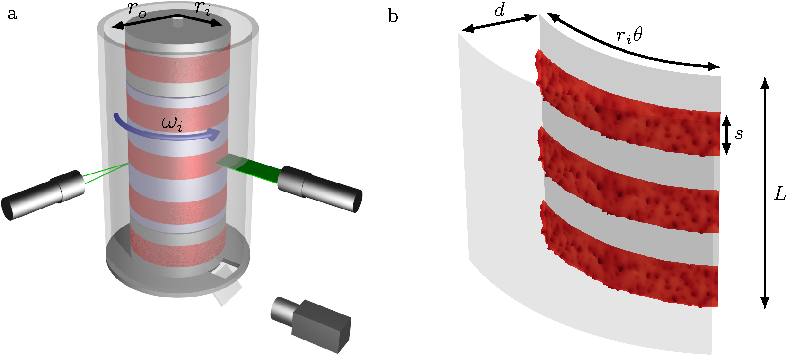
\includegraphics{fig2_setupnum.pdf}
\caption{a) Schematic of the Twente Turbulent Taylor--Couette showing the sandpaper on the inner cylinder in red. PIV measurements in the $r$--$\theta$ plane are illuminated from the side using a high-power laser creating a horizontal sheet. The sheet is imaged through a window in the bottom. Using LDA the azimuthal velocity is measured along the axial direction. The torque is measured in the middle section of the IC, which has a length of $\text{L}_{mid}=\SI{536}{\mm}$. b) Numerical domain for the case of $\tilde s\equiv s/d=0.47$, sandpaper roughness taken from the scan of the material used in the experiment, see \protect\reff{fig:roughness}.}
\label{fig:setupnum}
\end{figure}
%
\begin{figure}
    \centering
    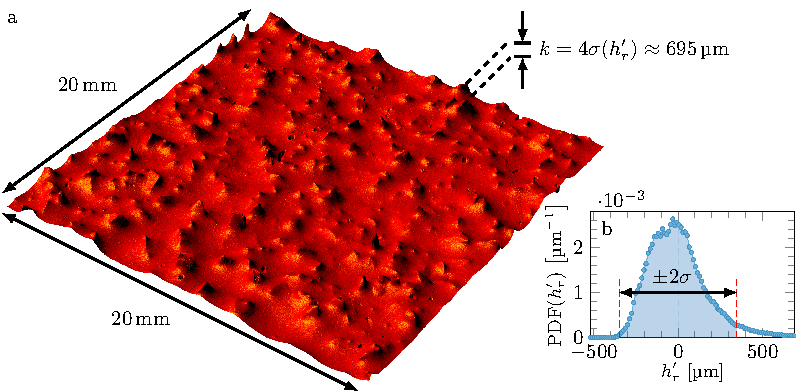
\includegraphics{fig1_roughness.pdf}
    \caption{a) Height scan captured using confocal microscopy of a roughness patch of \SI[product-units = repeat]{20 x 20}{\milli\metre} with a resolution of \SI{2.5}{\micro\meter}. The typical size of the grains is given by $k \equiv 4\sigma(h_r) = \SI{695}{\micro \meter}$ where $h_r$ is the height and $\sigma$ the standard deviation. The normalized typical grain size is then $k/d\approx 0.01$. b) Probability density function (PDF) of the measured height of the roughness patch, with subtracted mean $h_r' = h_r - \langle h_r \rangle$.}
    \label{fig:roughness}
\end{figure}%

\begin{table}
\centering
\begin{tabular}{cc}
Metric & Value \\
\hline
$\sigma(h_r) = \sqrt{\left \langle h_r'^2 \right \rangle}$ & \SI{174}{\micro\meter} \\
$\left \langle \left| h_r' \right| \right \rangle$ & \SI{134}{\micro\meter} \\
$\min(h_r')$ & \SI{-527}{\micro\meter} \\
$\max(h_r')$ & \SI{738}{\micro\meter} \\
$\mathrm{median}(h_r')$ & \SI{-19.6}{\micro\meter} \\
$\mathrm{mode}(h_r')$ & \SI{-27}{\micro\meter} \\
$\mathrm{IQR}=Q3-Q1=\mathrm{CDF}^{-1}(0.75)-\mathrm{CDF}^{-1}(0.25)$ & \SI{215}{\micro\meter} \\
$\left \langle h_r'^3 \right \rangle / \left \langle h_r'^2 \right \rangle^{3/2}$ & 0.928 \\
$\left \langle h_r'^4 \right \rangle / \left \langle h_r'^2 \right \rangle^2$ & 4.361 \\
wetted area/flat area & $\approx 1.6$
\end{tabular}
\caption{Various statistics of the roughness $h_r' = h_r - \langle h_r \rangle$ based on the data obtained from confocal microscopy, see also figure \protect{\ref{fig:roughness}}.}
\label{tbl:roughness}
\end{table}%
\clearpage
%%%%%%%%%%%%%%%%%%%%%%
%%%% Methods: TOK %%%%
%%%%%%%%%%%%%%%%%%%%%%
\subsubsection*{Global measurements: Torque}
We measured the torque, $\mathcal{T}$, that is required to drive the inner cylinder at constant angular velocity (the outer cylinder is kept at rest). For this we use a hollow flange reaction torque transducer connecting the driving shaft and the inner cylinder. We continuously measure the torque while quasi-statically ramping the frequency of the inner cylinder, $f_i$, from $\SI{5}{\hertz}$ to $\SI{18}{\hertz}$. This corresponds to $\text{Ta} \approx 4\times 10^{11}$ and $\text{Ta} \approx 6 \times 10^{12}$. All the experiments are performed at \SI[separate-uncertainty =
true,multi-part-units=single]{21(1)}{\celsius} and all quantities are calculated using the actual measured temperature. Table\,\ref{sim_param} shows additional experimental parameters.

%%%%%%%%%%%%%%%%%%%%%%%%%%%%%%%
%%%% Methods: LDA  and PIV %%%%
%%%%%%%%%%%%%%%%%%%%%%%%%%%%%%%
\subsubsection*{Local measurements: LDA and PIV}
We performed an axial scan of the azimuthal velocity with laser Doppler anemometry (LDA). The scan was performed at the middle of the gap, $\tilde{r}=(r-r_i)/d=0.5$, at a fixed $\text{Ta}=9.5\times 10^{11}$.
The flow was seeded using $\SI{5}{\mu \meter}$-diameter polyamide particles with density of \SI{1030}{\kilo\gram\per\metre\cubed} that act as tracers \citep{vanGils2012}.
The laser beam goes through the outer cylinder and is focused in the middle of the gap. We correct for curvature effects by numerically ray tracing the LDA beams as it was shown in \citet{Huisman2012}. The axial extent of the LDA scans is $0 \leq z/L \leq 0.5$.
Particle image velocimetry (PIV) measurements were performed at $\text{Ta}=9.5\times 10^{11}$ (same as LDA) in the radial-azimuthal plane. The scan is done for different heights and for different $\tilde{s}$.
The working fluid is seeded with PPMA fluorescent particles (\texttt{Dantec FPP-RhB-10}) with diameters of 1--\SI{20}{\micro\metre} with a seeding density of $\approx 0.01 \ \text{particles}/\text{pixel}$.
These particles have an emission peak at $\approx \SI{565}{\nm}$. We illuminate the particles with a \texttt{Quantel Evergreen 145} \SI{532}{\nano\meter}, double pulsed laser. A cylindrical lens is used to create a light sheet of $\approx \SI{1}{\mm}$ thickness. The images are captured with an \texttt{Imager SCMOS ($2560 \times  2160$ pixel) 16 bit} camera with a \texttt{Carl Zeiss 2.0/100} lens. The camera is operated in double frame mode with a frame rate $f$ which is always smaller than the interframe time $1/ \Delta t$, i.e. $\Delta t \ll 1/f$. In order to enhance the particle contrast in the images, we add a \texttt{Edmund High-Performance Longpass 550 nm} filter to the camera lens. For every $\tilde{s}$, the axial extent of the experiments is different. This is done because---as will be shown later---the aspect ratio of the rolls change depending on $\tilde{s}$. For the smallest $\tilde{s}=0.63$ however, the axial resolution is $\delta z/L \approx 0.011$ while for the largest value $\tilde{s}=3.74$, $\delta z / L\approx 0.022$. Since we scan in the axial direction, the focus of the camera is changed accordingly. The fields are resolved with a commercial PIV software (\texttt{Davis 8.0}) based on a multi-step method. The initial window size is set to $64\times 64 \ \text{pixels} $ and it decreases to $32\times 32$ pixels for the last iteration. The fields are calculated in cartesian coordinates, which we transform to polar coordinates. The final result is the fields in the form $\vec{u}=u_r(r,\theta,t)\hat{e_r}+u_\theta(r,\theta,t)\hat{e_\theta}$, where $u_r$ and $u_\theta$ are the radial and azimuthal velocity component which depend on the radius $r$, the azimuthal (streamwise) direction $\theta$ and time $t$.
%%%%%%%%%%%%%%%%%%%%%%%%%%%%%%%%%%%%%%%%%%%%%%%%
%%%%%%%%%%%%%% NUMERICAL METHODS %%%%%%%%%%%%%%%
%%%%%%%%%%%%%%%%%%%%%%%%%%%%%%%%%%%%%%%%%%%%%%%%
\subsection{Numerical methods}\label{sec:num_methods}
The Navier-Stokes (NS) equations are spatially discretized by using a central second-order finite-difference scheme and solved in cylindrical coordinates by means of a semi-implicit procedure \citep{Verzicco1996, vanderPoel2015}. The staggered grid is homogeneous in both the spanwise and streamwise directions (the axial and azimuthal directions, respectively). The wall-normal grid consists of double cosine (Chebychev-type) grid stretching. Below the maximum roughness height, we employ a cosine stretching such that the maximum grid spacing is always smaller than $0.5$ times the viscous length scale $\delta_\nu=\nu/u_\tau$. In the bulk of the fluid, we employ a second stretching, such that the maximum radial grid spacing in the bulk is  $\approx 1.7\delta_\nu$. The minimum radial grid spacing is $\approx 0.33 \delta_\nu$, and thus is located at the position of the maximum roughness height, where we expect the highest shear stress. In table\,\ref{sim_param}, we show a summary of the relevant parameters in the simulations. Time advancement is performed by using a fractional-step third-order Runge--Kutta scheme in combination with a Crank--Nicolson scheme for the implicit terms. The Courant--Friedrichs--Lewy (CFL) $(u\Delta t)/ (\Delta x)<0.8$ time-step constraint for the non-linear terms is enforced to ensure stability.
We scale the roughness patch such that the maximum roughness height, and thus the maximum blockage ratio, is max($h_r$)$=0.1d$. Depending on $\tilde{s}$, we cut out a portion of roughness from the scanned surface. The roughness is then mirrored and pasted together to obtain a smooth, streamwise periodic, stripe. Note that we do not mirror the surface in the spanwise direction. The streamwise and spanwise lengths of the computational domain are set to match the minimum computational domain size as studied in \cite{Ostilla-Monico2014b}.
A moving average over $10\times 10$ points is employed to smooth the scan from measurement noise. Finally, we set the resolution based on the demands ($\Delta z^+, r_i \Delta \theta^+ < 3$), which is small enough to recover the smallest geometrical features of the surface. 
The sandpaper roughness is implemented in the code by an immersed boundary method (IBM) \citep{Fadlun2000}. In the IBM, the boundary conditions are enforced by adding a body force $\mathbf{f}$ to the NS equations. A regular, non-body fitting, mesh can thus be used, even though the rough boundary has a very complex geometry. We perform interpolation in the spatial direction preferential to the normal surface vector to transfer the boundary conditions to the momentum equations. The IBM has been validated previously \citep{Fadlun2000, Iaccarino2003, Stringano2006, Zhu2016, Zhu2017, Zhu2018}. 
\ifdefined\thesissections
\begin{landscape}
\fi
\begin{table}
\centering
\hspace*{-0.0cm}\begin{tabular}{ccccc|ccc|ccccccccc}
$\tilde s$ & $N_\theta\times N_z \times N_r$ &$\text{Ta}$ & $\Gamma$  & $\text{Re}_\tau$ & $C_f$ & $\text{Nu}_\omega$ & $\Delta (\omega)^+$ &  $\Delta r^+_\text{min}$ & $\Delta r^+_\text{max}$\\
\hline
Simulations &  & $\times 10^9$ \\ 
\hline
smooth 	 & $758\times600\times840$  & $2.39$  & $2.08$& $697$  & $0.049$  &$30.1$  & $-$  & $0.28$  & $2.44$ & \\

uniformly rough& $1324\times 1012\times 1200$ & $1.19$ & $2.00$ & $689$ &$0.095$  & $41.5$ & $8.11$  & $0.33$  & $1.76$ \\
$0.47$   & $1324\times 1275\times 1200$ & $1.33$ & $2.52$ & $686$ &$0.084$  & $38.9$ & $6.36$  & $0.33$  & $1.76$ \\
$0.62$   & $1324\times 1121\times 1200$ & $1.33$ & $2.22$ & $690$ &$0.085$  & $39.4$ & $6.78$  & $0.33$  & $1.77$ \\
$0.93$   & $1324\times 1682\times 1200$ & $1.45$ & $3.32$ & $692$ &$0.079$  & $38.1$ & $6.21$  & $0.33$  & $1.77$ \\
$1.24$   & $1324\times 1121\times 1200$ & $1.37$ & $2.22$ & $685$ &$0.082$  & $38.3$ & $6.20$  & $0.33$  & $1.75$ \\

\hline
Experiments &  & $\times 10^{12}$ & & $\times 10^3$\\ 
\hline
smooth & & 1.00 & 11.7 & 10.1 & 0.024 & 307 & & & \\
0.61 & &$1.00$ & $11.7$   & $13.1$  & $0.041$ & $509$ & &  &\\
0.93 & &$1.00$ & $11.7$   & $13.5$  & $0.043$ & $534$ & &  &\\
1.23 & &$1.00$ & $11.7$   & $13.3$  & $0.041$ & $508$ & &  &\\
1.87 & &$1.00$ & $11.7$   & $12.9$  & $0.039$ & $491$ & &  &\\
3.74 & &$1.00$ & $11.7$   & $14.4$  & $0.049$ & $517$ & &  &\\
%Future: full rough and full smooth data
\hline

\multicolumn{8}{c}{} \\
\end{tabular}
\caption{List of parameters involved in both the simulations and the experiments. $\tilde{s}=s/d$ is the normalized roughness width. $N_\theta\times N_z \times N_r$ is the numerical resolution in the azimuthal, axial, and radial direction, respectively. $\Delta (\omega)^+$ is the downward shift of the angular velocity profile $\omega^+$. $\Delta r_{min}^+$ is the minimum spacing in the wall normal direction at the location of the maximum roughness height. $\Delta r_{max}^+$ is the maximum spacing in the wall normal direction. $r_i^+ \Delta \theta = \Delta z^+ \approx 2.7$ ($r_o^+ \Delta \theta \approx 3.8$) is the grid spacing in the streamwise and spanwise directions. In the DNS, the roughness height $k^+ = 4\sigma(h_r)^+ = 130 \pm 1$ for all rough cases. The roughness is glued to the surface and thus protruding, such that $r_k > r_i$, with $r_k$ the radial coordinate of the rough surface patches and $r_i$ the radial position of the smooth patches.}
\label{sim_param}
\end{table}
\ifdefined\thesissections
\end{landscape}
\fi

%%%%%%%%%%%%%%%%%%%%%%%%%%%%%%%%%%%%%%%%%%%%%%%%
%%%%%%%%%%%%%%%%%%% Results %%%%%%%%%%%%%%%%%%%%
%%%%%%%%%%%%%%%%%%%%%%%%%%%%%%%%%%%%%%%%%%%%%%%%
\section{Results}\label{sec:spanwiseresults}
%%%%%%%%%%%%%%%%%%%%%%%%%%%%%%%%%%%%%%%%%%%%%%%%
%%%%%%%%%% Results: Secondary flows %%%%%%%%%%%%
%%%%%%%%%%%%%%%%%%%%%%%%%%%%%%%%%%%%%%%%%%%%%%%%
\subsection{Response of the Turbulent Taylor Vortices}\label{sec:resultsec}
\begin{figure}
\centering
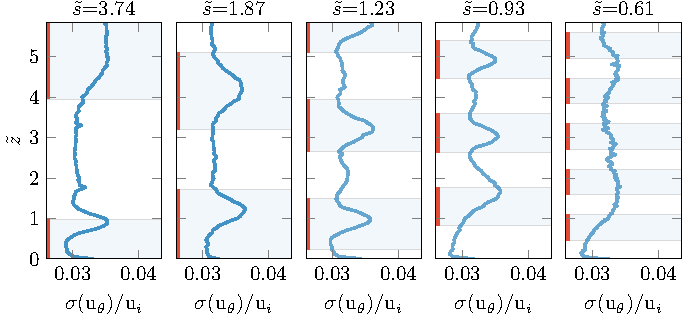
\includegraphics{fig3_ldaFluctuations.pdf}
\caption{%
Standard deviation of the azimuthal velocity $\sigma(u_\theta)$, normalized by the inner cylinder azimuthal velocity $u_i$, as a function of $\tilde {z}=z/d$ for various $\tilde{s}$.
$\Ta=\num{1e12}$ for all experiments.
The enforced roughness pattern is indicated in red and a light blue shade.
The signature of the roughness pattern is clearly visible at mid-gap in the bulk flow. For $\tilde s=0.61$, the roughness pattern shows does not leave a distinct imprint of its topology in the midgap flow statistics.}
\label{fig:explda}
\end{figure}
In order to get a first insight on the effect of the roughness on the flow, we performed axial scans of the azimuthal flow velocity at midgap using LDA.
Subsequently, we calculated the standard deviation of the azimuthal velocity. In \reff{fig:explda}, we show the standard deviation of the azimuthal velocity $\sigma(u_\theta)$ normalized with the inner cylinder velocity $u_i$, as a function of the height, for various $\tilde s$. Here, the axial coordinate is normalized using the height of the cylinders such that $\tilde z = z/d$. The standard deviation is a measure of the magnitude of the velocity fluctuations and therefore, we can now quantify the effect of the applied roughness. \refF{fig:explda} reveals that for the case of the largest patch size ($\tilde s=3.74$), the smooth section has, on average, a value of $\sigma(u_\theta)/u_i  \approx 0.03$, slightly larger than $\sigma(u_\theta)/u_i \approx 0.023$ that is found for the smooth case (for $\Ta=\num{1.5e12}$) in the same apparatus \citep{vanGils2012}. Above the rough section, towards the center of the setup (\text{i.e.} for large $\tilde z$), $\sigma(u_\theta)$ gradually increases to a value of approximately $\sigma(u_\theta)/u_i \approx 0.04$.
A similar, but not so clear trend can be seen at the lower roughness section ($\tilde z \approx 0.93$) of this case. However, this might be influenced by the lower bottom plate of the system.
When looking at the $\tilde s=1.87$ case, we see very similar, however more pronounced dynamics. Azimuthal velocity fluctuations are promoted in regions where the roughness is present, as suggested by the appearance of local peaks centered at the position of the rough patches. This effect is further seen for the cases of $\tilde{s}=1.23$ and $\tilde{s}=0.93$, where we clearly observe similar profiles. At their smooth areas however, we observe plateaus for $\sigma(u_\theta)$, similar to the ones for the $\tilde s=3.74$ case, although with a slightly higher value. For the final case with $\tilde s=0.61$ this trend seems to fade away and we see that $\sigma(u_\theta)$ becomes more axially independent, i.e. the peaks are less pronounced, and do not seem to follow the topology of the roughness patches.
The results from \reff{fig:explda} hints that the presence of the roughness might have an effect on the morphology of the flow, far away from the roughness sublayer region \citep{Berghout2018}, on the order of the gap width $d$, and reminiscent to what is found in studies of pipe and channel flow \citep{Koeltzsch2002,Chung2018}. To gain more insight into how the roughness alters the flow, we set out to measure the velocity field in the meridional plane using PIV at multiple heights.

\begin{figure}
\centering
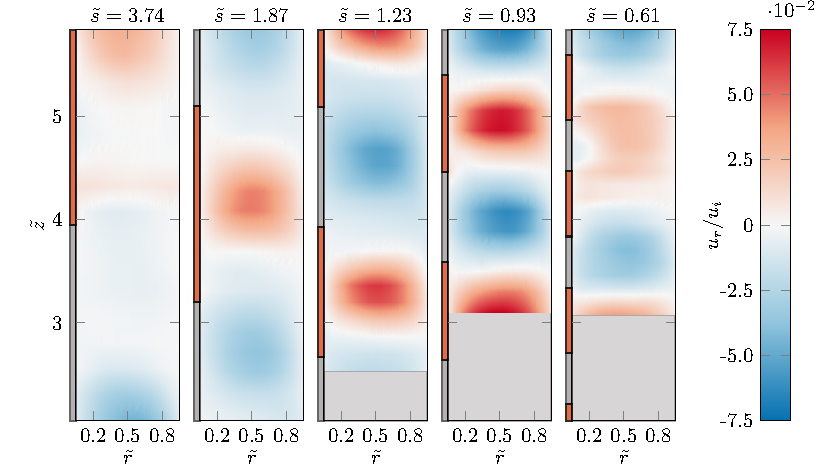
\includegraphics[width=0.99\textwidth]{fig4_pivRolls.pdf}
\caption{Temporal and azimuthal average of the radial velocity $u_r$, normalized with the inner cylinder azimuthal velocity $u_i$, obtained from PIV for varying roughness patch sizes $\tilde{s}$. A positive value of $u_r$ denotes outflow, while a negative value denotes inflow, with respect to the inner cylinder. It can be seen that the rolls are pinned by the roughness and their wavelength changes with $\tilde{s}$.
The red and gray areas at the left side of each plot indicate the positions of the rough and smooth areas, respectively.
Note that the typical grain size is $k/d \approx 0.01$. The gray shaded areas in the gap represent unexplored heights.}
\label{fig:exppiv}
\end{figure}

In figure \ref{fig:exppiv}, we show the temporal and azimuthally averaged radial velocity component $u_r$, normalized with $u_i$, in the spanwise wall-normal plane ($\tilde z$-$\tilde r$), where the radial coordinate is normalized such that $\tilde r = (r - r_i) / d$. \refF{fig:exppiv} shows that for the case of $\tilde{s}=3.74$, a very large structure can be seen, which consists of a large outflow region (positive $u_r$) around $\tilde{z}=5.84$, while a large inflow region (negative $u_r$) is detected around $\tilde{z}=2.10$. The situation is more pronounced for the cases of $\tilde{s}=1.87$, $\tilde{s}=1.23$, and $\tilde{s}=0.93$, where a clear roll-like  structure (i.e. the TTV) can be observed. Note that the radial component in the flow changes sign along the axial direction as it should in the presence of a TTV. What it is rather remarkable, is that the wavelength of the rolls $\lambda$ changes for different values of $\tilde{s}$. For the large structure at $\tilde{s}=3.74$, the normalized wavelength is $\tilde{\lambda}=\lambda/d \approx 4.01$. As $\tilde{s}$ decreases to $\tilde{s}=1.87$,  $\tilde{\lambda}\approx 1.49$.  At $\tilde{s}=1.23$, the wavelength decreases to a value of $\tilde{\lambda}\approx 1.42$. At $\tilde{s}=0.93$, $\tilde{\lambda}\approx 0.94$, and finally for the smallest value of  $s=0.61$, the wavelength increases slightly to $\tilde{\lambda}=1.09$. We remind the reader that the work of \citet{Huisman2014}, revealed that for counter-rotation ($a \approx 0.4$), the average wavelength of the rolls could be either $\tilde{\lambda}=1.46$ or $\tilde{\lambda}=1.96$ depending on the \textit{state} the system is in. The current work shows that by an appropriate choice of $\tilde{s}$, the wavelength of the rolls can firstly, abandon its natural state; and secondly, it can be tuned within the range $\tilde{\lambda}\in[0.94,4.01]$ by an appropriate choice of $\tilde{s}$. The wavelengths described above were calculated by measuring the locations of two consecutive maximum and minimum values of $\langle u_r \rangle_{t,\theta,r_{bulk}}$ along $z$ which are closest to midheight. Here, the symbol $\langle \cdot \rangle_{t,\theta,r_{bulk}}$ denotes average over time, the streamwise direction and the bulk region, i.e. $(r_{bulk}-r_i)/d\in[0.3,0.7]$.

In addition, we observe that outflow regions are created in axial regions where the roughness is located; and conversely, inflow regions are created in the smooth areas. Note that this  orientation of the secondary flows is opposite to what is found in other canonical systems (e.g. pipe flow and channel flow \citep{Willingham2014, Yang2017, Chung2018}), where one finds inflow regions above the rough patches and outflow region above the smooth patches. Another interesting observation is that because the driving is now from the BL rather than the bulk, the strength of the rolls change depending on the value of $\tilde{s}$, as evidenced by the magnitude of $|u_r|$. In order to explore this feature in more detail, we quantify the strength of the rolls with $\tilde{u_r}^\prime\equiv \sqrt{\langle (u_r/u_i)^2 \rangle_{t,\theta,r_{bulk},z_\lambda}}$ as a function of $\tilde{s}$. Here, the symbol $\langle \cdot \rangle_{t,\theta,r_{bulk},z_\lambda}$ denotes an average over time, the streamwise direction, the bulk region, and the axial region that defines the wavelength of a single roll $z_\lambda$. In \reff{fig:exptok}(c), we show $\tilde{u_r}^\prime$ as a function of $\tilde{s}$, where we observe that the strength of the rolls increases with decreasing $\tilde{s}$ for $\tilde{s}\in[0.93,3.74]$. However at $\tilde{s}=0.61$ the trend is broken, where we observe that $\tilde{u_r}^\prime$ decreases with respect to the case of $\tilde{s}=0.93$.

\begin{figure}
\centering
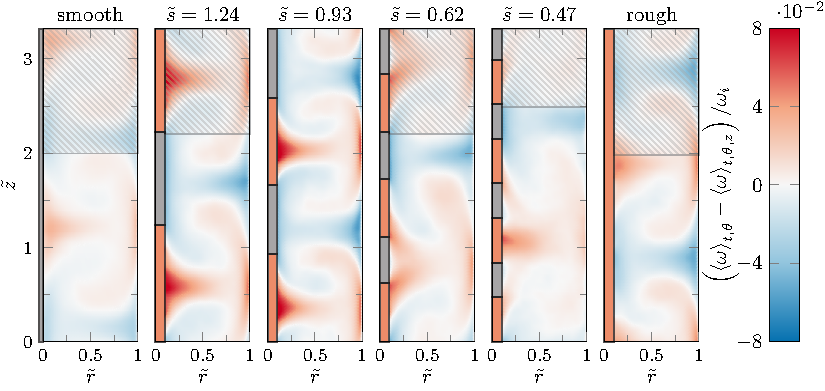
\includegraphics[width=0.99\textwidth]{fig6_simPlumes.pdf}
\caption{Deviation of the temporal and azimuthally averaged angular velocity $\langle \omega \rangle_{t,\theta}$ with respect to the temporal, azimuthal, and axial averaged angular velocity $\langle \omega \rangle_{t,\theta,z}$ obtained from DNS at $\text{Ta}\approx 1.0\times 10^{9}$, and for all $\tilde{s}$ explored in DNS. The fields are normalized with the inner angular velocity $\omega_i=u_i/r_i$. Positive values represent velocities that are closer to the IC velocity. The leftmost panel corresponds to the case of no roughness while the rightmost panel is the case where the entire IC is uniformly rough. Hatched regions are copied from the actual numerical domains---which are periodic in the axial direction---to allow for straightforward comparison. Ejecting regions can be seen in axial locations where the roughness is present. Notice the similarity of the structures with those found in the experiments shown in figure 6.}
\label{fig:simomega}
\end{figure}

In order to obtain more insight into the mechanism(s) that lead to the varying $\tilde{\lambda}$ for varying $\tilde{s}$, we turn to DNS, albeit at a much lower Ta ($\approx 1.0\times 10^9$), and much higher roughness height ($k/d \approx 0.1$). Since very large $\tilde s$ cases are not feasible for DNS, we focus on matching the exact $\tilde s$ in the lower range. We will show that, despite the O($10^3$) difference in $\text{Ta}$, the same observations found in the numerics are also found in the experiments. 

First, we look at the azimuthal velocity component. In \reff{fig:simomega}, we plot the difference of the temporal and azimuthal average of the angular velocity $\langle \omega^+ \rangle_{t,\theta}$ with respect to the temporal, azimuthal and,  axial average of the angular velocity $\langle \omega^+ \rangle_{t,\theta,z}$ in wall units. This is done to emphasize the underlying organization of the TTVs. Here, we clearly observe that for all $\tilde{s}$, ejecting regions of angular velocity are originated in the rough patches, similar to the preferential plume ejection sides at the tips of grooves in \citet{Zhu2016}. These ejecting regions advect fluid from the roughness patch on or at the inner cylinder towards the outer cylinder. As a consequence, an array of plume-like structures are formed along the axial direction. In TC flow (without roughness), plume-like structures are clear signatures of the presence of TTVs \citep{Ostilla-Monico2014b,Ostilla-Monico2014}. A closer inspection of \reff{fig:simomega} reveals that for the largest value of $\tilde{s}=1.24$, the plumes have enough separation such as not to interact between them. When $\tilde{s}$ is lowered to $\tilde{s}=0.93$, we observe that the plumes come closer, and can, in fact, begin to interact with each other. At the lower $\tilde{s}=0.62$ however, the situation is rather different. Here, one rough patch does not create a single plume as for the previous cases; a plume is created from the interaction of two ejecting regions. For the $\tilde{s}=0.47$ case, we observe finally that a plume-like structure is originated from three different rough patches. The behavior of the plumes for $\tilde{s}=0.62$, and $\tilde{s}=0.47$ is the result of the merging of the plumes that arise from the roughness patches. These observations help us to rationalize the change in the wavelength and strength of the rolls shown in \reff{fig:exppiv}. If $\tilde{s}$ decreases, the plumes are effectively forced to come closer to each other; and as a result, the roll changes its wavelength and becomes stronger due to the added interaction of the plumes. In \reff{fig:pivomega} we show $(\langle \omega \rangle_{t,\theta}-\langle \omega \rangle _{t,\theta,z})/\omega_i$, the same quantity discussed previously, albeit now for the experiments. Here, we can clearly see that a similar mechanism takes place. Plume-like structures are originated at the centers of the roughness elements and interact with each other if the spacing (small $\tilde{s}$) is reduced. 

\begin{figure}
\centering
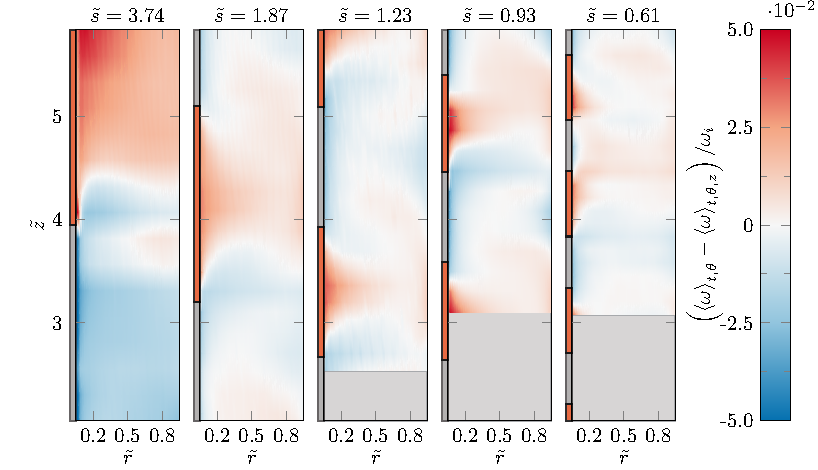
\includegraphics[width=0.99\textwidth]{fig5_omegafluc.pdf}
\caption{Deviation of the temporal, and azimuthal averaged angular velocity $\langle \omega \rangle_{t,\theta}$ with respect to the temporal, azimuthal, and axial averaged angular velocity $\langle \omega \rangle_{t,\theta,z}$ obtained from the experiments at $\text{Ta}=9.5\times 10^{11}$, and for all $\tilde{s}$ explored in experiments. The fields are normalized with the inner angular velocity $\omega_i=u_i/r_i$. Ejecting regions can be seen in axial locations where the roughness is present. Notice the similarity of the structures with those found in the numerics shown in figure 5. }
\label{fig:pivomega}
\end{figure}

The LDA, PIV and DNS explored in this section reveal that there is a mean effect of the spanwise-varying roughness on the large scale secondary flows that exist in turbulent TC flow. We have seen thus far that the roughness pins the rolls, and that their wavelength and strength can be tuned depending of the choice of $\tilde{s}$ over a wide range of $\text{Ta}$, and a wide range of roughness heights $h$. However, how does the flow respond globally, i.e. the angular momentum transport, to this change in morphology? This will be addressed in the following section.

%%%%%%%%%%%%%%%%%%%%%%%%%%%%%%%%%%%%%%%%%%%%%%%%
%%%%%%%%%% Results: Global response %%%%%%%%%%%%
%%%%%%%%%%%%%%%%%%%%%%%%%%%%%%%%%%%%%%%%%%%%%%%%
\subsection{Global response}
\label{sec:resultglob}

\begin{figure}
\centering
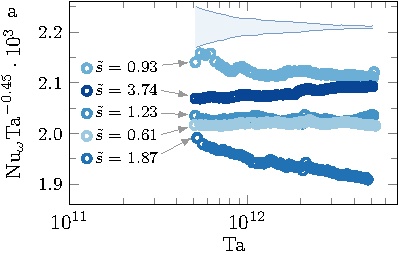
\includegraphics[width=0.49\textwidth]{fig8a_tanuw.pdf}
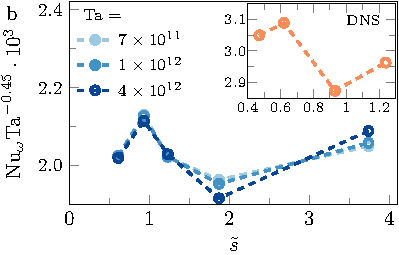
\includegraphics[width=0.49\textwidth]{fig8b_sdnuw.pdf}\\
\vspace{2mm}%
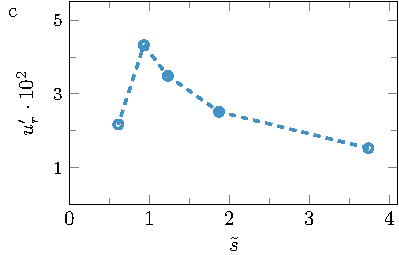
\includegraphics[width=0.49\textwidth]{fig8c.pdf}
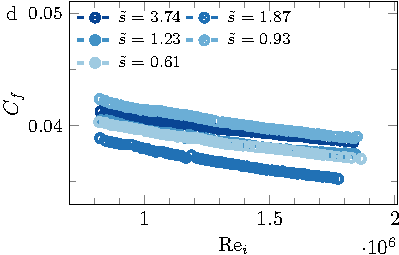
\includegraphics[width=0.49\textwidth]{fig8d_sdcf.pdf}
\caption{(a) Compensated Nusselt number $\text{Nu}_\omega\text{Ta}^{-0.45}$ as a function of $\text{Ta}$ for varying $\tilde{s}$. The shaded area indicates the error of the measurements, which can be seen to decrease with increasing driving. (b) Compensated Nusselt number $\text{Nu}_\omega\text{Ta}^{-0.45}$ as a function of $\tilde{s}$ for 3 selected \text{Ta}. Here, an optimum value in the transport of angular momentum is observed close to $s/d \approx 1$. The inset in (b) shows the results obtained with the DNS, where the maximum can be observed at a lower $\tilde{s}$, namely $\tilde{s}\approx 0.6$. (c) Normalized RMS of the radial velocity $u_r^\prime$ as a function of $\tilde{s}$, obtained from the PIV experiments. (d) Friction coefficient $C_f$ as a function of the driving, expressed with the Reynolds number $\text{Re}_i$, for various $\tilde{s}$.}
\label{fig:exptok}
\end{figure}

The global response of the TC system can be expressed with the $\text{Nu}_\omega$ (\ref{eq:spanwisenu}). In \reff{fig:exptok}(a), we show the compensated Nusselt number as a function of the driving, where a scaling of $\text{Nu}_\omega\propto \text{Ta}^\alpha$, with $\alpha=0.45$ is revealed for all the $\tilde{s}$ explored; except for $\tilde{s}=1.87$, where the scaling is closer to $\alpha=0.44$. In the absence of roughness and within the same range of Ta, the scaling is found to be effectively $\text{Nu}_\omega\propto \text{Ta}^{0.40}$ \citep{Paoletti2011,vanGils2011,Huisman2014}.
In contrast, when both of the solid walls are made uniformly rough (i.e. pressure drag dominates), the scaling asymptotes to the ultimate regime scaling famously predicted by Kraichnan, \textit{i.e.} $\text{Nu}_\omega\propto \text{Ta}^{0.5}$ \citep{Kraichnan1962,Zhu2018}. In  \cite{Zhu2018}, the closest configuration to our study is the case of rough IC and smooth OC, for which the exponent $\alpha=0.43$ is found. We note that this exponent is somewhat smaller than the ones observed in the current study. The reason behind this, is currently unknown. We notice, however, that the roughness type in our study is rather different. In this study we use spanwise-varying sandgrain roughness, while the roughness in \citet{Zhu2018} is made of rib obstacles and is oriented along the streamwise direction. 

In order to connect the observed dynamics of the TTVs with the global response, we plot in \reff{fig:exptok}(b), the compensated Nusselt number $\text{Nu}_\omega \Ta^{-0.45}$ as a function of $\tilde{s}$ for both the experiments and the numerics. We note that that the exponent found for $\tilde{s}=1.87$ ($\alpha=0.44$) is nearly the same as $\alpha=0.45$. We see rather remarkably, the appearance of a maximum around $\tilde{s}\approx 0.93$ for the experiments, and $\tilde{s} = 0.61$ for the DNS. We attribute the appearance of this peak to the strengthening of the TTVs, which is caused by the variation of $\tilde{s}$, and thus of $\tilde{\lambda}$. Explicitly, by lowering $\tilde{s}$, we can lower the wavelength of the rolls and bring them closer together (see \refsec{sec:resultsec}). As a consequence, the rolls are strengthened which leads to an enhancement of the angular momentum transport; and thus, the peak around $\tilde{s} = 0.93$. This occurrence is also observed by \citet{Huisman2014}, although the mechanism observerd there is quite different. While the rolls in their study are enhanced by counter-rotating the OC; in our case, the rolls are strengthened by forcing $\tilde{s}$ below their natural wavelength due to the right choice of the spanwise varying roughness. This is also supported by the observation that the magnitude of the radial velocity shows a maximum around $\tilde{s}=0.93$, as shown in \reff{fig:exptok}(c). We note, however, that the torque is not measured throughout the entire axial length of the cylinders $L=\SI{927}{\mm}$, but in a smaller section of length $L_{\text{mid}}=\SI{536}{\mm}$. As a result, the large structure identified previously for the case of $\tilde{s}=3.74$ ($\tilde{\lambda}=4.01$), does not fit entirely in the measurement section (see the first panel of \reff{fig:exppiv}). As a a result, the Nusselt number that corresponds to this case, could be under or overestimated.

We also note that in the case of the numerics, the position of the maximum is different than in the experiments. We attribute this to a combination of two effects. On the one hand the DNS is performed at a lower Ta, which has an effect on the natural wavelength of the rolls as it was shown by \citet{Chouippe2014}, who show that for similar values of $\eta$, the wavelength of the rolls can decrease with decreasing Ta. On the other hand, the axial domain of the DNS is bounded by $\Gamma\in[2.08,3.32]$, which gives rise to limited box-sizes. Thus, when $\tilde{s}$ is varied, the rolls could suffer from an additional $\textit{constraint}$ due to the limited axial domain. In addition to this discrepancy, we also note that the scaling in the range of Ta at which the DNS is done ($\approx 1.0\times 10^9$), is not known a priori. Since no other exponent is presently available to us, we chose to compensate the numerical data with the same exponent found in the experiments (\reff{fig:exptok}(b)). However, we note that this exponent might be different due to the $2$ decades of separation  in Ta between the numerics and experiments, as was also shown by \citet{Zhu2018}. We would like to emphasize, however, that in spite of these discrepancies, a maximum in angular momentum transport is observed for a given $\tilde{s}$ in both the experiments and the numerics, which is solely a consequence of the varying axial wavelength of the TTV, dictated by the spanwise-varying roughness.


%%%%%%%%%%%%%%%%%%%%%%%%%%%%%%%%%%%%%%%%%%%%%%%%
%%%%%%%%% Results: Velocity profiles %%%%%%%%%%%
%%%%%%%%%%%%%%%%%%%%%%%%%%%%%%%%%%%%%%%%%%%%%%%%
\subsection{Velocity profiles}
\label{sec:results_velprofiles}

\begin{figure}
\centering
  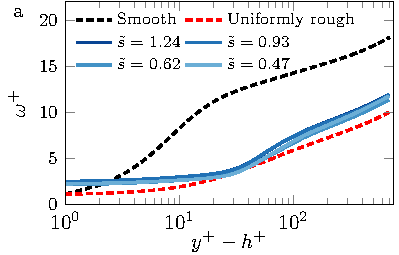
\includegraphics[width=0.49\linewidth]{fig9a_omegaplus.pdf}
  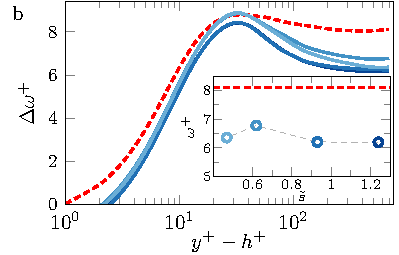
\includegraphics[width=0.49\linewidth]{fig9b_d0.pdf}
\caption{
(a) Angular velocity $\omega^+$ profiles versus the wall normal distance $y^+-h_m^+$ for various $\tilde{s}$, where $h_m^+$ is the virtual origin and equals the melt-down (i.e. mean) height of the rough surface. The solid black line represents the uniformly rough case. (b) Angular velocity shift $\Delta \omega^+$ as a function of $y^+-h^+$ for varying $\tilde s$. In the inset of (b), we show the angular velocity shift $\Delta \omega^+$ versus the wall normal distance $y^+-h_m^+$. Here, we observe a maximum downwards shift of the angular velocity profile for the simulation where we cover the entire inner cylinder with sandpaper roughness (i.e. uniformly rough). }
\label{fig:o_do}
\end{figure}

Having discussed the dynamics of the TTVs and the corresponding global response, in terms of the dimensionless torque, we now set out to study the streamwise, angular, velocity profiles (rather than the azimuthal profiles, as discussed in \cite{Grossmann2014} and \cite{Berghout2018}). To allow for straightforward comparison between the respective velocity profiles, we run the DNS at constant friction Reynolds number $Re_\tau = 690 \pm 10$. The profiles are then temporally, azimuthally, and axially averaged $\omega^+ = \langle \omega \rangle_{t,\theta,z}/\omega_\tau$. The profiles still exhibit a logarithmic region when averaged over the entire axial coordinate. \reff{fig:simomega} shows however that the TTVs in the flow, following the spanwise-varying roughness, do not exhibit any outer similarity. Deviations of the azimuthal and temporal averages from the mean logarithmic profiles are found up to $\Delta \omega^+ \approx 2$. 

For turbulent flows over rough walls, the streamwise velocity profiles retains its logarithmic form. However, the hallmark effect of rough walls is a downwards shift of this region (for any drag increasing surface), which can also be understood as an increase of the skin friction factor $C_f$ \citep{Hama1954}. \refF{fig:o_do}(a) shows the angular velocity profiles $\omega^+$ as a function of  $(y^+-h_m^+)$, where $h_m^+$ is the virtual origin and equals the melt-down (i.e. mean) height of the rough surface. We choose the melt-down height of the roughness over the full inner cylinder as the virtual origin. In \reff{fig:o_do}(b) we show the velocity shift versus the wall normal distance. The inset gives a vertical cut at $y^+ = Re_\tau$. It is evident that also in this representation, an optimum in the velocity shift, and thus in  $C_f$ can be observed. The position of this maximum ($\tilde s = 0.61$) is the same as the one obtained from the angular momentum transport (see \refsec{sec:resultglob}).

%%%%%%%%%%%%%%%%%%%%%%%%%%%%%%%%%%%%%%%%%%%%%%%%
%%%%%%%%%%%% Conclusion & Outlook %%%%%%%%%%%%%%
%%%%%%%%%%%%%%%%%%%%%%%%%%%%%%%%%%%%%%%%%%%%%%%%
\FloatBarrier
\section{Conclusions and outlook}
\label{sec:conclusions}
In this study, we investigate, both numerically and experimentally, large Taylor number Taylor--Couette flow in the presence of spanwise-varying roughness, which consists of an arrangement of patches of width $\tilde s = s/d$, with $d$ the gap width, that covers the entire circumference of the inner cylinder. In the experiments, the patches are made from sandpaper, while in the numerics a confocal microscopy scan of the surface is implemented by means of the immersed boundary method (IBM). 

Remarkably, we find that by varying $\tilde s$ in the domain $\tilde s = [0.61, 3.74]$ we can alter the axial wavelength  of the turbulent Taylor vortices within the range $\tilde{\lambda}\in[0.94,4.01]$, even if the roughness height is very low ($k/d\approx 0.01$). This manipulation is observed to hold in a range of 3 decades in Ta ($\mathcal{O}(10^9)-\mathcal{O}(10^{12})$).

In the experiments, the scaling of the Nusselt number with the driving is found to be effectively $\text{Nu}_\omega\propto \text{Ta}^{0.45}$ for $\text{Ta}\in[5\times 10^{11},5\times 10^{12}]$); except for $\tilde{s}=1.87$, where a very similar exponent is found ($\alpha=0.44$). The experiments also revealed that inflow regions ($u_r<0$) originate between the rough patches, where the inner cylinder is hydrodynamically smooth (in contrast to secondary flows induced by spanwise-varying roughness in channel flow, where the orientation of the vortices is reversed \citep{Chung2018}. Conversely, at the center of the rough patches, we observe the creation of outflow regions ($u_r>0$) which are accompanied by the promotion of azimuthal velocity fluctuations $\sigma(u_\theta)$ at midgap. At these axial locations (center of rough patches), we observe, in both the numerics and experiments, the emission of plume-like structures, which are responsible for the creation and pinning of the rolls. Since the coverage of the roughness is fixed, we show that by reducing $\tilde{s}$, we can effectively bring these structures closer, and enhance the interaction of the rolls, as evidenced by the increment in $|u_r|$. As a consequence of this interaction, the flow responds globally by inducing a maximum of angular momentum transport at $\tilde{s}=0.93$ in the experiments, and $\tilde{s}=0.62$ in the numerics.  

We highlight that in this study, the change in the morphology of the large-scale structures is only due to the spanwise-varying roughness (of very low height) and not by a change of $\Gamma$ or $\eta$, which opens the possibility of exploring different configurations in which the rolls can be tuned at such large turbulence levels. 
 
Many questions arise from the aforementioned observations. Understanding the mechanisms leading to the merging of plume ejection regions, and accompanied parameter boundaries at which this occurs, would lead to a further insight into the dynamics of the TTVs. Furthermore, it would be intriguing, in the spirit of \citet{Bakhuis2018b}, to study the influence of spanwise-varying regions of idealized high and low wall shear stress, without geometrical induced disturbances. It is an open question whether one could also alter $\lambda$, without the interaction of the plumes.



%%%%%%%%%%%%%%%%%%%%%%
%%%% chapter done %%%%
%%%%%%%%%%%%%%%%%%%%%%
\graphicspath{{fig/}}
